% rubber : module pdftex
\documentclass{beamer}
%\usetheme{Berkeley}
%\usetheme{Antibes}
\usetheme{CambridgeUS}
\usecolortheme{dolphin}

\title%[SE390] % (optional, only for long titles)
{SE464 Project Deliverable 1 Presentation}
\subtitle{Group 17}
\author[SE2018] % (optional, for multiple authors)
{Software Engineering Class of 2018}
\institute[UW] % (optional)
{
  University of Waterloo
}
\date%[KPT 2004] % (optional)
{September 29, 2016}
\subject{Software Engineering}

%%% BEGIN PREAMBLE

\usepackage{geometry}
% \geometry{screen}
\title{Shots Fired}
\author{scmaier, d2lal, samiskin, wcakeize}

%%% BEGIN DOCUMENT
\begin{document}
\maketitle
\begin{frame}
\frametitle{Brief Project Description}
%  \begin{center}
%  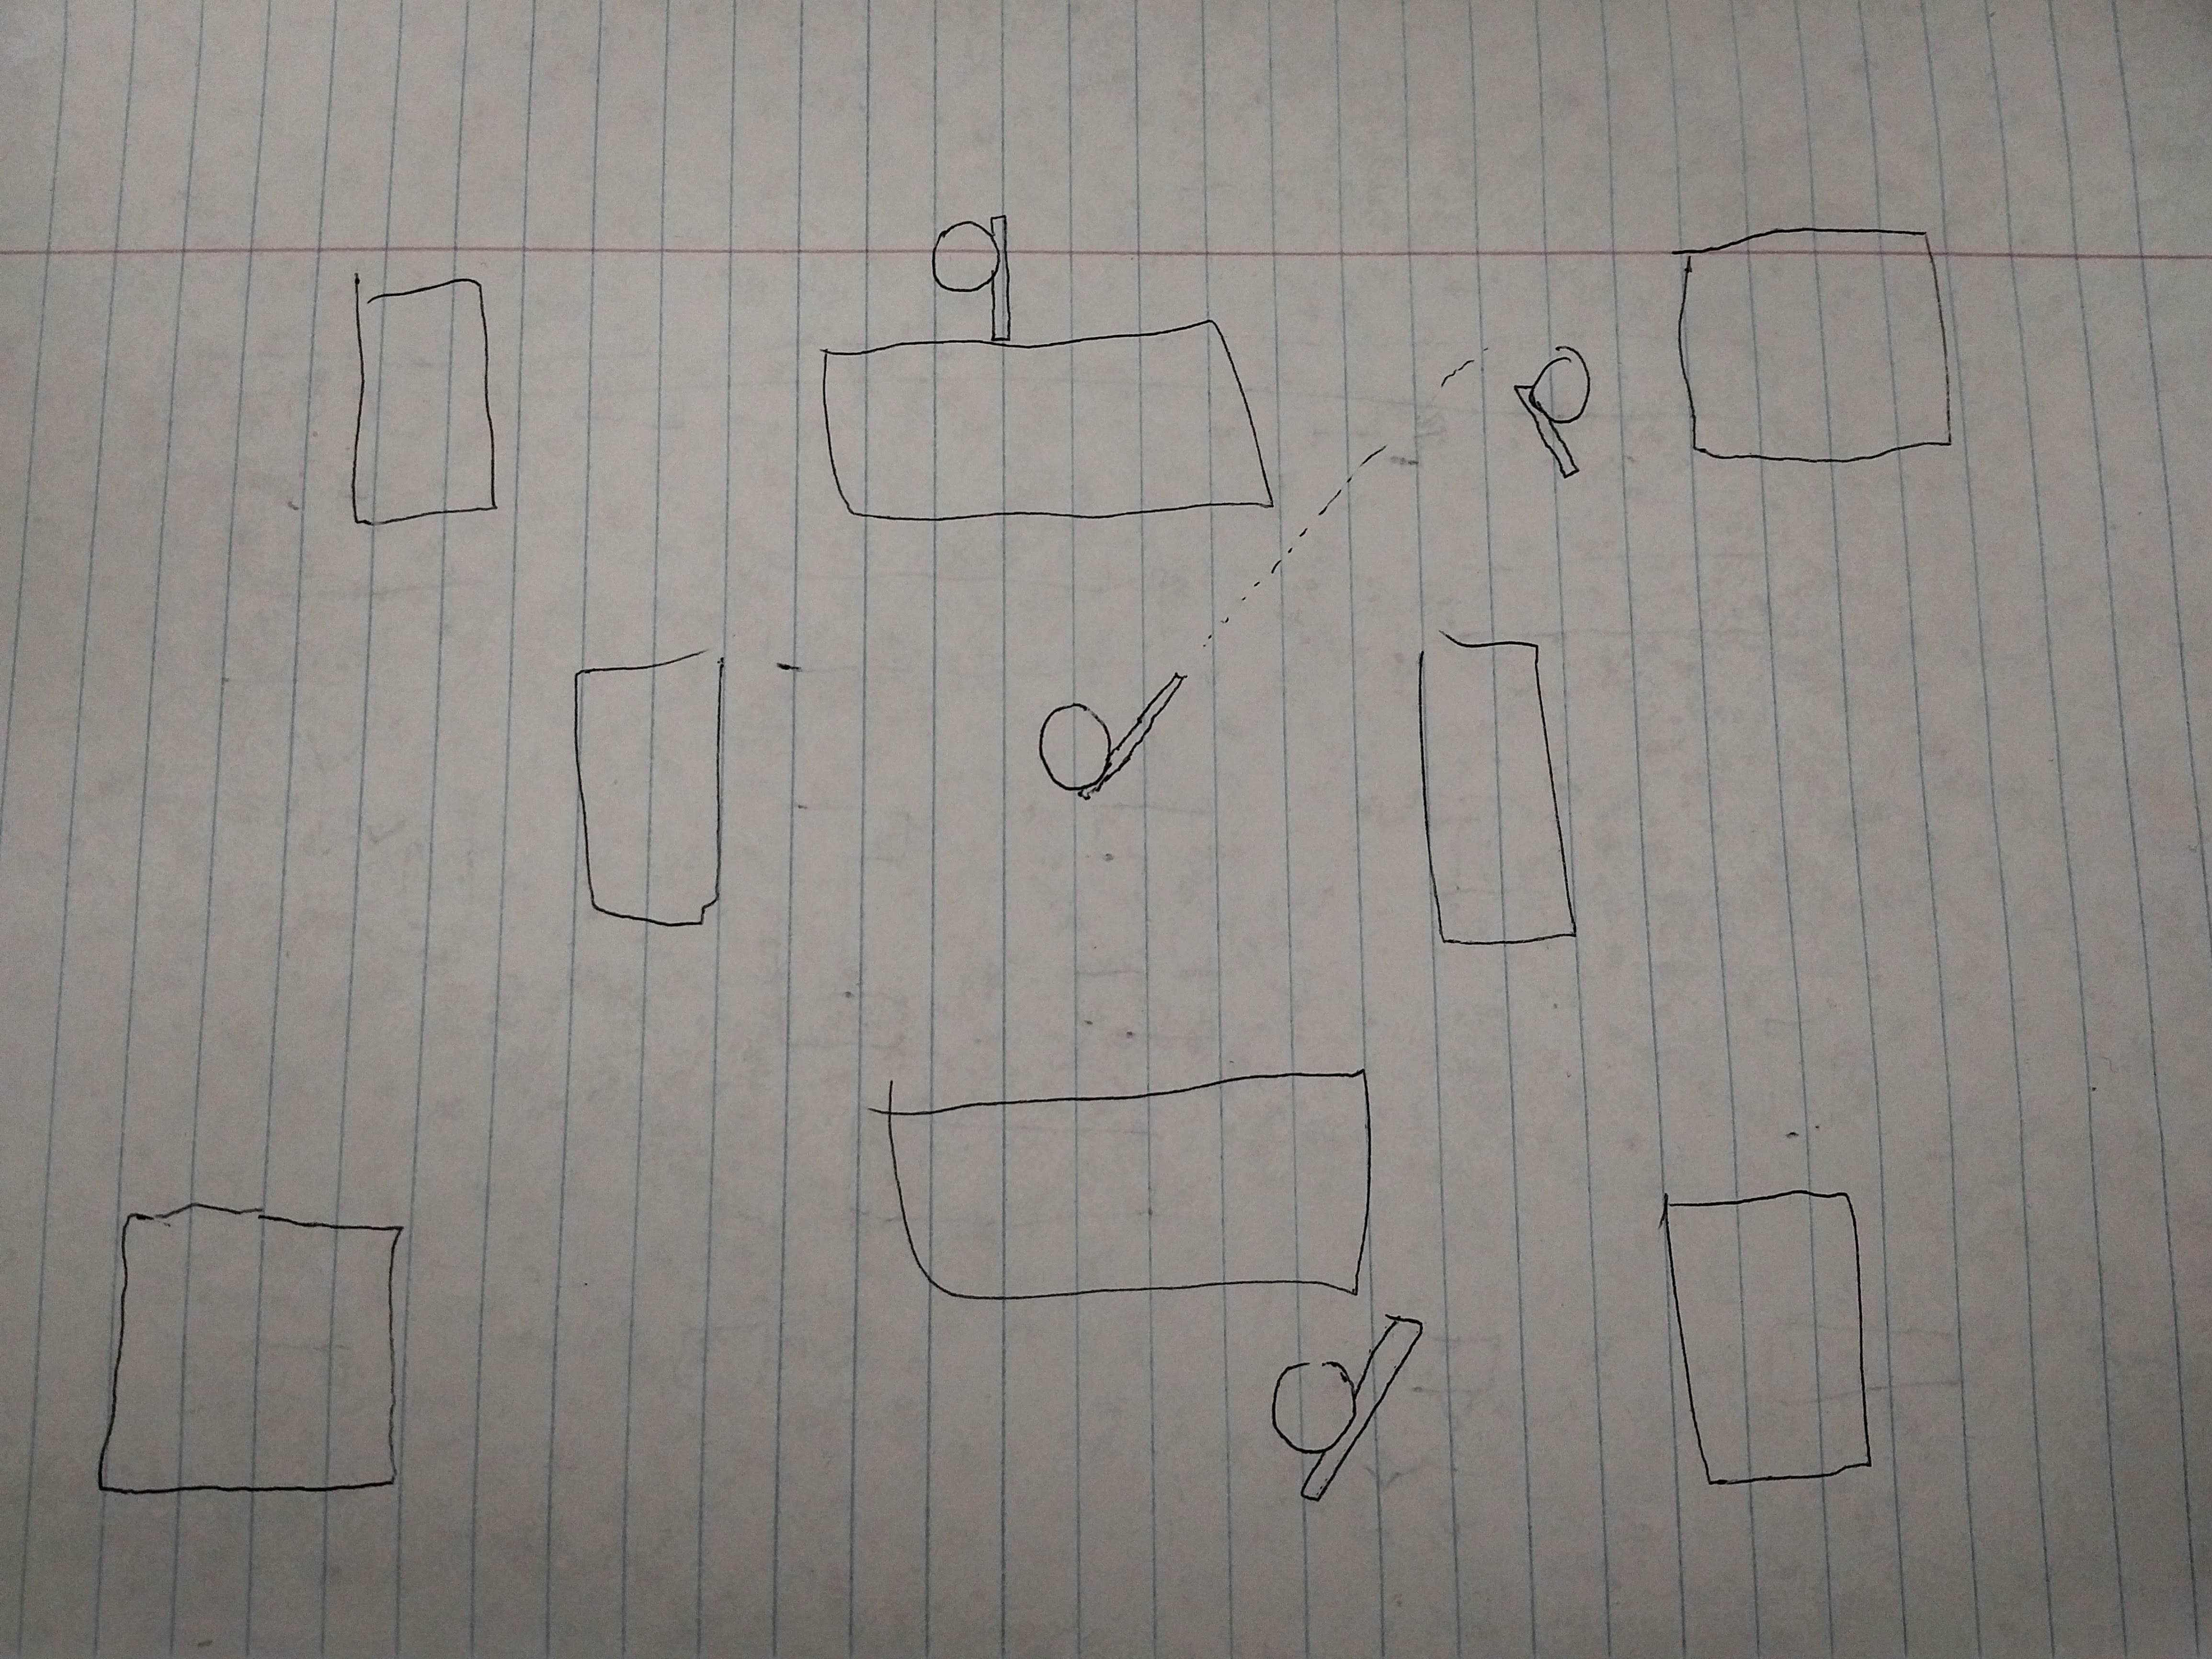
\includegraphics[scale=0.06]{images/mockup.jpg}
%  \end{center}
\begin{enumerate}
  \item Top-down arena style 2D multiplayer shooting game
  \item 2-4 player game played on separate machines connected online
  \item Characters are controlled with Keyboard and Mouse
  \item When a player loses all their health they are out
  \item Last person standing wins!
\end{enumerate}
\end{frame}

\begin{frame}
\frametitle{Game Mode 1: Quick Play}
\begin{enumerate}
  \item Player clicks the 'Quick Play' option in the main menu
  \item They are put in a lobby, waiting until more people have joined
  \item Once there are at least 2 players in the lobby, a countdown starts
  \item Countdown resets every time a new player joins the lobby
  \item If the countdown reaches 0 or the max number of players (4) have joined, the game starts
\end{enumerate}
\end{frame}

\begin{frame}
\frametitle{Game Mode 2: Private Match}
\begin{enumerate}
  \item Player clicks the 'Private Match' option in the main menu
\end{enumerate}
\end{frame}

\begin{frame}
\frametitle{Gameplay}
\begin{enumerate}
  \item Each player has x amount of health
\end{enumerate}
\end{frame}

\begin{frame}
\frametitle{End of Game}
\begin{enumerate}
  \item If the user won, they are presented with a winners screen
  \item If the user lost, they are presented with a game over screen
\end{enumerate}
\end{frame}

\begin{frame}
\frametitle{Design Challenges}
\begin{enumerate}
  \item TO CHANGE
  \item Creating a game with character interactions, animations, controls, physics, online connections
  \item Synchronizing differences between client and server game states
  \item Running and managing multiple game servers simultaneously
\end{enumerate}
\end{frame}

\begin{frame}
\frametitle{Requirements}
\begin{enumerate}
  \item TO REMOVE POSSIBLY
  \item Top-down arena style 2D shooting game
  \item 2-4 player game played on separate machines connected online
  \item Characters are controlled with Keyboard and Mouse
  \item Can easily join a game with friends (low barrier to entry)
\end{enumerate}
\end{frame}

\end{document}

